% Options for packages loaded elsewhere
\PassOptionsToPackage{unicode}{hyperref}
\PassOptionsToPackage{hyphens}{url}
\PassOptionsToPackage{dvipsnames,svgnames,x11names}{xcolor}
\documentclass[
  11pt,
]{article}
\usepackage{xcolor}
\usepackage[margin=25mm]{geometry}
\usepackage{amsmath,amssymb}
\setcounter{secnumdepth}{-\maxdimen} % remove section numbering
\usepackage{iftex}
\ifPDFTeX
  \usepackage[T1]{fontenc}
  \usepackage[utf8]{inputenc}
  \usepackage{textcomp} % provide euro and other symbols
\else % if luatex or xetex
  \usepackage{unicode-math} % this also loads fontspec
  \defaultfontfeatures{Scale=MatchLowercase}
  \defaultfontfeatures[\rmfamily]{Ligatures=TeX,Scale=1}
\fi
\usepackage{lmodern}
\ifPDFTeX\else
  % xetex/luatex font selection
\fi
% Use upquote if available, for straight quotes in verbatim environments
\IfFileExists{upquote.sty}{\usepackage{upquote}}{}
\IfFileExists{microtype.sty}{% use microtype if available
  \usepackage[]{microtype}
  \UseMicrotypeSet[protrusion]{basicmath} % disable protrusion for tt fonts
}{}
\makeatletter
\@ifundefined{KOMAClassName}{% if non-KOMA class
  \IfFileExists{parskip.sty}{%
    \usepackage{parskip}
  }{% else
    \setlength{\parindent}{0pt}
    \setlength{\parskip}{6pt plus 2pt minus 1pt}}
}{% if KOMA class
  \KOMAoptions{parskip=half}}
\makeatother
\usepackage{longtable,booktabs,array}
\usepackage{caption}
\captionsetup[table]{skip=6pt}
\newcounter{none} % for unnumbered tables
\usepackage{calc} % for calculating minipage widths
% Correct order of tables after \paragraph or \subparagraph
\usepackage{etoolbox}
\makeatletter
\patchcmd\longtable{\par}{\if@noskipsec\mbox{}\fi\par}{}{}
\makeatother
% Allow footnotes in longtable head/foot
\IfFileExists{footnotehyper.sty}{\usepackage{footnotehyper}}{\usepackage{footnote}}
\makesavenoteenv{longtable}
% definitions for citeproc citations
\NewDocumentCommand\citeproctext{}{}
\NewDocumentCommand\citeproc{mm}{%
  \begingroup\def\citeproctext{#2}\cite{#1}\endgroup}
\makeatletter
 % allow citations to break across lines
 \let\@cite@ofmt\@firstofone
 % avoid brackets around text for \cite:
 \def\@biblabel#1{}
 \def\@cite#1#2{{#1\if@tempswa , #2\fi}}
\makeatother
\newlength{\cslhangindent}
\setlength{\cslhangindent}{1.5em}
\newlength{\csllabelwidth}
\setlength{\csllabelwidth}{3em}
\newenvironment{CSLReferences}[2] % #1 hanging-indent, #2 entry-spacing
 {\begin{list}{}{%
  \setlength{\itemindent}{0pt}
  \setlength{\leftmargin}{0pt}
  \setlength{\parsep}{0pt}
  % turn on hanging indent if param 1 is 1
  \ifodd #1
   \setlength{\leftmargin}{\cslhangindent}
   \setlength{\itemindent}{-1\cslhangindent}
  \fi
  % set entry spacing
  \setlength{\itemsep}{#2\baselineskip}}}
 {\end{list}}
\usepackage{calc}
\newcommand{\CSLBlock}[1]{\hfill\break\parbox[t]{\linewidth}{\strut\ignorespaces#1\strut}}
\newcommand{\CSLLeftMargin}[1]{\parbox[t]{\csllabelwidth}{\strut#1\strut}}
\newcommand{\CSLRightInline}[1]{\parbox[t]{\linewidth - \csllabelwidth}{\strut#1\strut}}
\newcommand{\CSLIndent}[1]{\hspace{\cslhangindent}#1}
\setlength{\emergencystretch}{3em} % prevent overfull lines
\providecommand{\tightlist}{%
  \setlength{\itemsep}{0pt}\setlength{\parskip}{0pt}}
\usepackage{bookmark}
\IfFileExists{xurl.sty}{\usepackage{xurl}}{} % add URL line breaks if available
\urlstyle{same}
% fallback for those not using the hyperref driver hyperxmp:
\makeatletter
\@ifundefined{xmpquote}{\newcommand{\xmpquote}[1]{#1}}{}
\makeatother
\hypersetup{
  pdftitle={HGFX supplementary evidence and provenance},
  pdfauthor={Mohammad Ahmadkhanloo},
  colorlinks=true,
  linkcolor={Maroon},
  filecolor={Maroon},
  citecolor={Blue},
  urlcolor={Blue},
  pdfcreator={LaTeX via pandoc}}

\title{Online Resource 1: HGFX: reference-compatible hierarchical Gaussian filtering in Python}
\author{Mohammad Ahmadkhanloo}
\date{9 November 2026}

\setlength{\emergencystretch}{3em}
\usepackage{graphicx,caption}
\renewcommand{\figurename}{Fig.}
\captionsetup[figure]{labelfont=bf,labelsep=space}
\renewcommand{\thefigure}{S\arabic{figure}}
\begin{document}
\maketitle

Computational Statistics\\
Mohammad Ahmadkhanloo\\
Institute for Research in Fundamental Sciences (IPM), Tehran, Iran\\
Correspondence: m.ahmadkhanloo@ipm.ir



\subsection{S1 Frozen identities and
regeneration}\label{s1-frozen-identities-and-regeneration}

The evaluated HGFX release is 1.0.0. Its source commit is

\texttt{4dd8fbd8239d05f2c7932a9a9b3b7795f0a9ab27}.

The MATLAB oracle is 8.2.0 at

\texttt{2437f4dc241541072722a2695ddeca7b44d83dd3}. These identities
define the scope; current development features are not included.
Original recovery experiments were not rerun. A new, prospectively
bounded released-wheel demonstration uses empirical exchange-rate
inputs; it is kept separate from frozen parity evidence.

Candidate figures regenerate with \texttt{python\ generate\_figures.py}
from this directory. The agreement/accuracy figure is redesigned from
the frozen decision; recovery is redrawn in grayscale from the decision,
and pyhgf includes a signed residual from all frozen trials. Horizon and
backend figures are byte-identical copies of historical images.
Input/output hashes and manuscript claims are indexed in the repository
ledger. The workflow diagram is conceptual and contains no data.
Complete machine-readable source links appear in the repository claim
ledger; this supplement supplies a compact reading route.

\subsection{S2 Fitting and recovery}\label{s2-fitting-and-recovery}

The official stress fit D02 and holdout D08 retain endpoint/inference
failures. In D02, a localized shared-vector objective difference was
\(2.842170943040401\times10^{-14}\); the state discrepancy was zero and
the maximum trial-likelihood difference was
\(8.881784197001252\times10^{-16}\). Six of six MATLAB one-spacing start
perturbations changed optimizer endpoints. For D08, 13 of 14 such
perturbations moved the endpoint outside its unchanged gate. These are
exact-scope reference-sensitivity findings, not direct endpoint parity
or an explanation for the separate P3 initial-fit failures. The
historical M18 scientific failure remains separate from paired S7
accounting.

The paired grid has 72 parameter cases and 36 model-recovery datasets
with three candidate fits each. There are 12 shards, two trial lengths
(128,256), two truth scales (0.15,0.35 prior SD), six parameter
replicates per stratum and three model replicates per stratum. The
selection rule is minimum BIC. Metrics rounded for display; full
precision remains in the frozen decision:

{\def\LTcaptype{none} % do not increment counter
\begin{minipage}{\linewidth}
\begin{tabular}{@{}
  >{\raggedright\arraybackslash}p{(\linewidth - 8\tabcolsep) * \real{0.2000}}
  >{\raggedright\arraybackslash}p{(\linewidth - 8\tabcolsep) * \real{0.2000}}
  >{\raggedright\arraybackslash}p{(\linewidth - 8\tabcolsep) * \real{0.2000}}
  >{\raggedright\arraybackslash}p{(\linewidth - 8\tabcolsep) * \real{0.2000}}
  >{\raggedright\arraybackslash}p{(\linewidth - 8\tabcolsep) * \real{0.2000}}@{}}
\toprule\noalign{}
\begin{minipage}[b]{\linewidth}\raggedright
Model
\end{minipage} & \begin{minipage}[b]{\linewidth}\raggedright
Implementation
\end{minipage} & \begin{minipage}[b]{\linewidth}\raggedright
Convergence
\end{minipage} & \begin{minipage}[b]{\linewidth}\raggedright
Median r
\end{minipage} & \begin{minipage}[b]{\linewidth}\raggedright
Median sRMSE
\end{minipage} \\
\midrule\noalign{}


hgf\_binary & matlab & 0.833333333333 & 0.202684570158 &
2.60966284547 \\
hgf\_binary & hgfx & 0.833333333333 & 0.202684570141 & 2.60966284551 \\
ehgf\_binary & matlab & 0.916666666667 & 0.461918369101 &
2.35912688823 \\
ehgf\_binary & hgfx & 0.916666666667 & 0.461918369078 & 2.35912688867 \\
uhgf\_binary & matlab & 0.791666666667 & 0.380968313583 &
2.95788661965 \\
uhgf\_binary & hgfx & 0.791666666667 & 0.380968313591 & 2.95788661807 \\
\bottomrule
\end{tabular}
\end{minipage}

}

The frozen scientific criteria are convergence \textgreater=0.80, median
r \textgreater=0.50, median sRMSE \textless=1.00 and model-recovery
balanced accuracy \textgreater=0.50. Agreement is 36/36 winners, while
balanced accuracy is 0.5833333333333334 in each implementation. These
are deterministic grid summaries, not uncertainty intervals.

\subsubsection{S2.1 Parameter-wise
recovery}\label{s2.1-parameter-wise-recovery}

The combined transformed-vector indices are 12, 13 and 14 (zero-based):
omega2, omega3 and log zeta. Each row below pools 24 cases, including
returned nonconverged fits. Values come from the original aggregate
archive, whose SHA-256 matches the digest in the retained S7 decision.
No new fitting was performed.

{\def\LTcaptype{none} % do not increment counter
\begin{minipage}{\linewidth}
\begin{tabular}{@{}llll@{}}
\toprule\noalign{}
Model & Parameter & r MATLAB / HGFX & sRMSE MATLAB / HGFX \\
\midrule\noalign{}


hgf & omega2 & 0.988404 / 0.988404 & 0.155871 / 0.155871 \\
hgf & omega3 & -0.396490 / -0.396490 & 2.771273 / 2.771273 \\
hgf & log zeta & 0.202685 / 0.202685 & 2.609663 / 2.609663 \\
ehgf & omega2 & 0.732432 / 0.732432 & 1.006879 / 1.006879 \\
ehgf & omega3 & 0.145726 / 0.145726 & 2.398578 / 2.398578 \\
ehgf & log zeta & 0.461918 / 0.461918 & 2.359127 / 2.359127 \\
uhgf & omega2 & 0.970916 / 0.970916 & 0.245734 / 0.245734 \\
uhgf & omega3 & 0.198098 / 0.198098 & 3.170042 / 3.170042 \\
uhgf & log zeta & 0.380968 / 0.380968 & 2.957887 / 2.957887 \\
\bottomrule
\end{tabular}
\end{minipage}

}

The per-parameter scale is the population standard deviation (ddof=0) of
its 24 generated transformed truths, not the prior standard deviation or
a standard error. sRMSE divides RMSE by this scale, except for the
historical fallback scale of one if the standard deviation is at most
\(10^{-12}\). The median correlation excludes nonfinite correlations;
the median sRMSE includes all three parameters. These deterministic
perturbation-grid summaries are not population confidence intervals. The
grid's truth rule is a sinusoidal perturbation of transformed prior
means at two scales, not an independent random population sample.

\subsubsection{S2.2 Model recovery confusion
matrix}\label{s2.2-model-recovery-confusion-matrix}

Both implementations have the same row-normalized matrix. Rows are
generating models; columns are selected models. There are 12 datasets
per generating model. Counts below are recovered exactly from the
original proportions and denominator.

{\def\LTcaptype{none} % do not increment counter
\begin{minipage}{\linewidth}
\begin{tabular}{@{}llll@{}}
\toprule\noalign{}
Generating model & Selected HGF & Selected eHGF & Selected uHGF \\
\midrule\noalign{}


HGF & 4/12 & 2/12 & 6/12 \\
eHGF & 0/12 & 11/12 & 1/12 \\
uHGF & 4/12 & 2/12 & 6/12 \\
\bottomrule
\end{tabular}
\end{minipage}

}

Balanced accuracy is \((4/12+11/12+6/12)/3=0.5833333333333334\). The
eHGF diagonal differs substantially from the other two, which a single
accuracy value conceals. Source: evidence/s7\_aggregate.json; the
archived ZIP is retained so access does not depend on an Actions
artifact remaining online.

\subsection{S3 Trial-horizon integrity and retrospective
localization}\label{s3-trial-horizon-integrity-and-retrospective-localization}

The original run 35272347167 contains 24 shards, 144 parameter cases and
72 model cases. Its frozen gate remains false. The 24 original shard
archives were reacquired and verified against GitHub archive digests.
The original checker, aggregator and diagnostic sources are retained
from execution commit \texttt{a051e747a3a60054159c81a8b8405fb4b2398277}.
The new audit only classifies existing records; it does not modify that
run or re-estimate parameters.

{\def\LTcaptype{none} % do not increment counter
\begin{minipage}{\linewidth}
\begin{tabular}{@{}
  >{\raggedright\arraybackslash}p{(\linewidth - 4\tabcolsep) * \real{0.3333}}
  >{\raggedright\arraybackslash}p{(\linewidth - 4\tabcolsep) * \real{0.3333}}
  >{\raggedright\arraybackslash}p{(\linewidth - 4\tabcolsep) * \real{0.3333}}@{}}
\toprule\noalign{}
\begin{minipage}[b]{\linewidth}\raggedright
Recorded outcome
\end{minipage} & \begin{minipage}[b]{\linewidth}\raggedright
Cases
\end{minipage} & \begin{minipage}[b]{\linewidth}\raggedright
Interpretation
\end{minipage} \\
\midrule\noalign{}


Matching nonempty model selections & 62 of 72 & Same selected model \\
No selected model in either implementation & 10 of 72 & Invalid
generation, not different winners \\
Two different nonempty selected models & 0 of 72 & None observed;
original full-grid gate still fails \\
Shared invalid parameter-case simulations & 20 of 144 & No fitted
parameter pair \\
HGFX initial rejection / MATLAB return & 4 of 144 & Asymmetric
execution; see below \\
Successful parameter-fit pairs & 120 of 144 & All recorded free-index
vectors match the expected vector \\
\bottomrule
\end{tabular}
\end{minipage}

}

The checker defines winner\_match as equality AND a nonempty selection.
Its free-index test compares returned vectors with the expected vector
even when a fit did not run or failed and returned an empty vector. Thus
24 index-contract failures comprise the 20 shared invalid simulations
and four asymmetric cases. They do not demonstrate reordering among
successful pairs. The aggregator uses global coverage and winner
conditions for each family's diagnostic label; the three mismatch labels
are not three independently localized model defects.

The four asymmetric cases all use classic HGF, truth scale 0.35, at the
two longer horizons. HGFX records an unstable initial objective before
entering optimization. MATLAB marks a function return successful even
when its objective is nonfinite. The recorded cases are:

{\def\LTcaptype{none} % do not increment counter
\begin{minipage}{\linewidth}
\begin{tabular}{@{}
  >{\raggedright\arraybackslash}p{(\linewidth - 6\tabcolsep) * \real{0.2500}}
  >{\raggedright\arraybackslash}p{(\linewidth - 6\tabcolsep) * \real{0.2500}}
  >{\raggedright\arraybackslash}p{(\linewidth - 6\tabcolsep) * \real{0.2500}}
  >{\raggedright\arraybackslash}p{(\linewidth - 6\tabcolsep) * \real{0.2500}}@{}}
\toprule\noalign{}
\begin{minipage}[b]{\linewidth}\raggedright
Trials
\end{minipage} & \begin{minipage}[b]{\linewidth}\raggedright
Replicate (zero-based)
\end{minipage} & \begin{minipage}[b]{\linewidth}\raggedright
MATLAB negative log joint
\end{minipage} & \begin{minipage}[b]{\linewidth}\raggedright
HGFX stage
\end{minipage} \\
\midrule\noalign{}


512 & 0 & negative infinity & Initial objective rejected \\
512 & 4 & 247.25740970068986 & Initial objective rejected \\
1024 & 0 & negative infinity & Initial objective rejected \\
1024 & 4 & 620.4345219314272 & Initial objective rejected \\
\bottomrule
\end{tabular}
\end{minipage}

}

The control-flow boundary is localized to the initial-objective
admissibility check in the recovery fitting routine, not to a
demonstrated optimizer endpoint competition. Historical records do not
contain the paired intermediate states needed to identify the first
divergent trial, level and variable, or to decide whether the two finite
MATLAB cases reflect a semantic or numerical difference. No root-cause
correction or universal fit-equivalence claim is made. The long-horizon
grid stays excluded from the supported paired-fitting claim; reproducing
or repairing it requires a separately frozen diagnostic exercise.

The retained generator errors report invalid variational approximation.
The ten absent winners are counted as unsuccessful cases, not discarded.
Row-normalized confusion matrices in the historical P3 aggregate
normalize selectable models only; their accuracy must not be read as
all-case success. This is another reason not to use those diagnostic
accuracies as an identifiability result.

\begin{center}
\begin{minipage}{\linewidth}
\centering
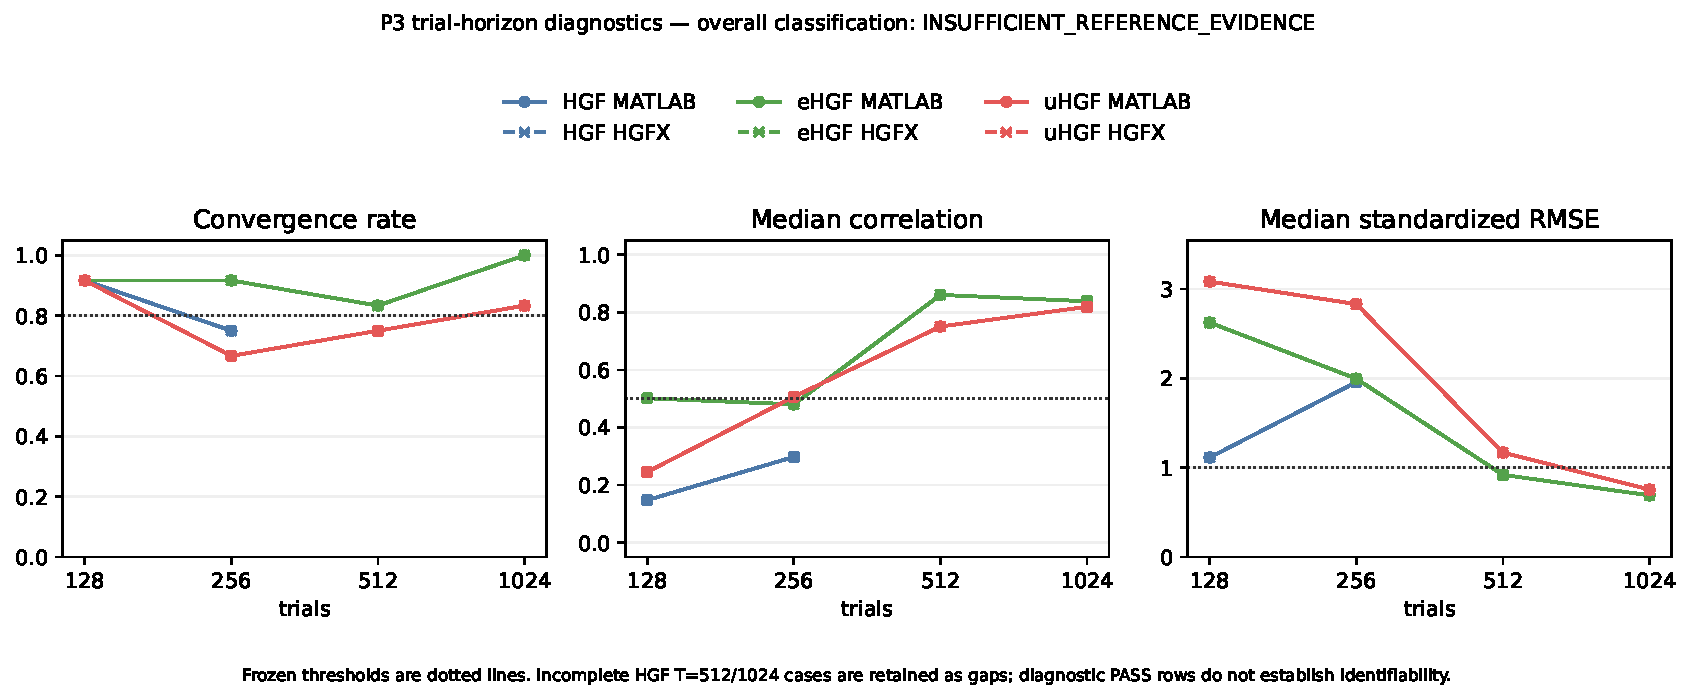
\includegraphics[width=\linewidth]{FigS1.pdf}
\captionof{figure}{Historical diagnostic recovery metrics by horizon, retained without changing values. Dotted lines are frozen thresholds and gaps preserve invalid classic-HGF cases. The full-grid integrity gate fails. The retrospective audit distinguishes missing outputs from conflicting finite selections; it does not promote any plotted subset to a scientific success}
\end{minipage}
\end{center}

\subsection{S4 Backend applicability}\label{s4-backend-applicability}

Physical evidence is retained from source
\texttt{07b45a569e04e8e71244c5310dd2cc53dbb2b0ec}, Python 3.12.13,
JAX/JAXLIB 0.11.1. Two Tesla T4 devices were visible; four required
fitting cells ran on cuda:0. Residency checks and enumeration are
separate. Its raw JSON and retention basis remain archived; it is not a
new post-remediation GPU execution. The CPU remeasurement has its own
source/runtime identity. The maximum gaps are 0.006783711260709424
(compatibility/JAX CPU, criterion 0.10) and 1.4210854715202004e-14 (JAX
CPU/T4, criterion 1e-7).

\begin{center}
\begin{minipage}{\linewidth}
\centering
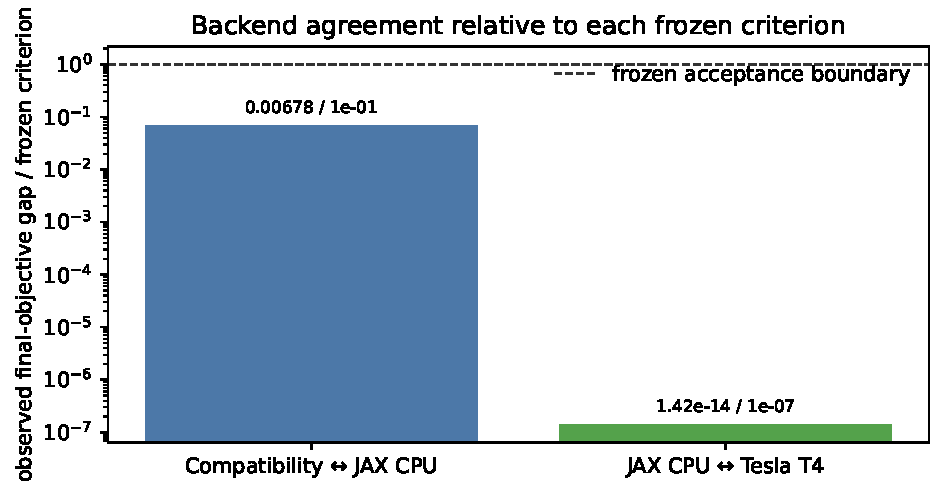
\includegraphics[width=\linewidth]{FigS2.pdf}
\captionof{figure}{Each maximum objective gap divided by its own frozen criterion; the dashed line is the acceptance boundary. These bars describe numerical agreement in recorded cells, without error bars. There is no speed measurement}
\end{minipage}
\end{center}

\subsection{S5 pyhgf common scope}\label{s5-pyhgf-common-scope}

pyhgf 0.3.2 source is \texttt{ccd43db5ee5abe4a5a35077d098e53cce2c070c2}.
The fixed 128-trial case uses a three-level binary hierarchy, standard
volatility updates and mean-field updates, zero drift and unit coupling.
The native response inverse temperature is 48. Input and response hashes
and the prospective semantic mapping remain in the original common-scope
record. Field-wise measured errors:

{\def\LTcaptype{none} % do not increment counter
\begin{minipage}{\linewidth}
\begin{tabular}{@{}lll@{}}
\toprule\noalign{}
Quantity & Classification & Maximum absolute error \\
\midrule\noalign{}


derived first level input surprise & PASS & 4.440892098500626e-16 \\
derived first level prediction error & PASS & 1.1102230246251565e-16 \\
first level predicted probability & PASS & 1.1102230246251565e-16 \\
level 2 posterior mean & PASS & 4.440892098500626e-16 \\
level 2 posterior precision & PASS & 6.661338147750939e-16 \\
level 2 predicted mean & PASS & 4.440892098500626e-16 \\
level 2 predicted precision & PASS & 6.661338147750939e-16 \\
level 3 posterior mean & PASS & 1.1102230246251565e-16 \\
level 3 posterior precision & PASS & 1.5543122344752192e-15 \\
level 3 predicted mean & PASS & 1.1102230246251565e-16 \\
level 3 predicted precision & PASS & 1.5543122344752192e-15 \\
participant response nll per trial & NDC & not applicable \\
participant response nll total & NDC & not applicable \\
\bottomrule
\end{tabular}
\end{minipage}

}

NDC applies to participant-response NLL at a probability boundary;
belief agreement does not repair the response comparison. No clipping or
changed tolerance was introduced after results. Package-wide or
fitted-model equivalence is untested.

\subsection{S6 Empirical example and published-study
boundaries}\label{s6-empirical-example-and-published-study-boundaries}

The input file is \texttt{demo/example\_usdchf.txt} from the frozen HGF
Toolbox 8.2.0 commit. The upstream demo identifies it as USD/CHF rates
during 2010/2011. The series has 614 finite values. Its original
market-data provider and individual calendar labels are not supplied in
this example, so the plots use observation number and do not claim
independent market-data verification. The included copy retains the
toolbox's MIT license and notice.

Protocol \texttt{REVISION\_PROTOCOL.md} was committed as
\texttt{a25690a} before execution. An isolated hgfx==1.0.0 wheel
environment ran the whole series outside the checkout with Python
3.12.10, JAX 0.11.1, NumPy 2.5.3, CPU and x64 enabled. The call uses
empty responses, hgf\_config, bayes\_optimal\_config and
quasinewton\_optim\_config, matching the official continuous-input
workflow. The likelihood is
\(\log p(u_t)=-\frac12\log(2\pi\hat\sigma_{1,t}^2)
-(u_t-\hat\mu_{1,t})^2/(2\hat\sigma_{1,t}^2)\). No response parameters
are fitted. Defaults resolve input-dependent priors from the first
observation and first 20 inputs; they are not hand-selected here.

The returned negative log likelihood is -2387.6219521878747, negative
log joint -2378.7708383887175, BIC -4736.723934806867 and approximate
LME 2376.7070907350367. Execution took 182.001 seconds on this
workstation. These are descriptive values from one execution, not a
speed benchmark or comparison with a null model. Ridders numerical
differentiation emitted invalid-subtraction warnings during the run. The
public result did not expose a termination-reason field; convergence and
Hessian quality are therefore not certified by the finite returned
statistics. No replacement optimizer, repeated fit or alternative prior
was tried.

Full transformed parameters, all 614 predicted/posterior state rows,
package identity, input digest and command are retained in
empirical\_example/. Figure 5 uses the observed series and those saved
states. Fitting used the full series, so predictions are conditional
in-sample diagnostics, not a held-out test. No independent MATLAB
comparison was executed for this new example.

The earlier 24-trial synthetic smoke test remains available in
worked\_example/. Its wheel acquisition used a mirror after the primary
host failed DNS resolution; wheel bytes were checked against the
official PyPI hash. The empirical run reuses that isolated environment
rather than importing the active development checkout.

Pain source commit is \texttt{3f1d32aff73826a1385c359ca638ad0e11a7fda7}.
Its input audit resolved the apparent filename discrepancy, but
custom-response permission and the historical environment remain open.
Some simulation files have GPL notices; no unlicensed custom source was
translated into HGFX. SPIRL source commit is
\texttt{86fd5122a744acfb5bc7ba12720426d8b4aa0ffa}; its custom eHGF and
seven joint choice/RT models require separate migration. Its 399 random
starts and original MATLAB R2019b settings were not silently simplified.
Neither study was fitted. The exchange-rate example adds empirical-input
use but does not close external participant-study replication. Upstream
participant files remain local and ignored.

\clearpage

\subsection{S7 Published behavioral input
validation}\label{s7-published-behavioral-input-validation}

The comparison used the two source files below. The preparation code
verified their SHA-256 digests before deriving the exact source-defined
block inventory.

\begin{itemize}
\tightlist
\item
  Suthaharan dataset (Suthaharan et al. 2021), 130 participant prefixes
  and 260 blocks.
  \href{https://github.com/psuthaharan/covid19paranoia/blob/c618e032228fb4ed03821f11bdc57af608695631/data/hgfPRL/pandemic_prelockdown_TP117_TP261_130.mat}{Pinned
  source file}.
\item
  Reed dataset (Reed et al. 2020), 32 participant prefixes and 64
  condition halves.
  \href{https://github.com/ModelDBRepository/258631/blob/39ccaca508b81ca610e7666a613e061c801faaf9/IRL_Data.mat}{Pinned
  source file}.
\end{itemize}

The
\href{https://github.com/ahmadkhanloo/hgfx/actions/runs/41809479255}{initial
source gate} rejected the assumed 326-block inventory before full-cohort
filtering. The MATLAB variable \texttt{ans} was outside the participant
schema. The corrected protocol fixed the 324-block population before
running the paired scientific computation. It retained all observed
source blocks and applied the union of missing-choice and
missing-outcome indices as the ignored-trial mask.

The perceptual model was \texttt{hgf\_ar1\_binary\_mab}, with three
arms, uncoupled updates and regular intervals. The native vector was
\((\mathrm{NaN},0,1,\mathrm{NaN},0.1,1,\mathrm{NaN},0,0.2,\mathrm{NaN},0,1,1,1,\mathrm{NaN},-2,-6)\).
The workflow used MATLAB R2025b Update 7 and the HGF Toolbox 8.2.0
source identified in S1, and the released HGFX 1.0.0 wheel with CPU
binary64. It compared complete trajectories and inference states with
the inherited tolerances of \(2\times10^{-9}\) relative and
\(2\times10^{-11}\) absolute. Matched nonfinite entries were included in
the array-entry count.

The
\href{https://github.com/ahmadkhanloo/hgfx/actions/runs/41809919116}{executed
run} retained all 324 comparison outcomes and exported an
\href{https://github.com/ahmadkhanloo/hgfx/actions/runs/41809919116/artifacts/13311622738}{aggregate
and status artifact}. The
\href{https://github.com/ahmadkhanloo/hgfx/blob/2dedd1dcf102ecc598f9151c2dc3ed6933c8c494/paper/case_studies/REALDATA_FORWARD_PARITY_RESULT_2026-11-04.md}{protocol,
source digests, environment and result} are recorded with the
reproduction code. The summary counts 48 blocks with Python warnings.
Participant inputs and per-trial outputs were excluded from the public
artifact.

The archived summary was retrieved again during the 8 November editorial
revision. Its ZIP SHA-256 was verified as
\texttt{1adfd1cd69b6f7d7a89ba2c8b9d564e774fd8a8841fa7243d6972605bd9f7391}.
The unchanged JSON member, retained at
\texttt{evidence/published\_input\_41809919116.json}, has SHA-256
\texttt{47432c35aa4914a652a8f1dc2aad81dc4d76fb5175dd0fc1fd47532b81756b70}.
This retrieval verifies the aggregate record. The underlying per-trial
comparisons were performed in the recorded workflow.

\subsection{S8. Bounded diagnostic and application follow-up (8 November
2026)}\label{s8.-bounded-diagnostic-and-application-follow-up-8-november-2026}

Recounting the archived 324-block status records found 86 warning events
in 48 Reed blocks: 29 blocks had one event and 19 had three. All 48
blocks included ignored trials. This association does not establish a
warning mechanism. The retained aggregate omits warning messages,
categories and source locations, and contains no trialwise arrays with
which to reassess nonfinite masks. No fresh MATLAB or HGFX execution is
claimed here. The original fixed-vector comparison remains unchanged;
harmlessness of the warnings is not established.

A bounded source feasibility check considered Oberwelland before Gao,
without fitting either. Oberwelland's public fitting script uses the
softmax\_binary observation configuration, which is outside the released
HGFX 1.0.0 public fitting dispatch. Its OSF file metadata returned HTTP
410 in this attempt. Gao's OSF file metadata returned HTTP 401; critical
source files could not be inspected. Access failures are session
observations, not evidence of permanent source unavailability. Neither
candidate qualified for the conditional application phase; models were
not substituted and participants were not selected by results. These
findings are source-audit outcomes, not additional participant-study
replications.

Machine-readable count and source-access records accompany the
repository handoff as publication\_completion\_audit\_20261108.json and
publication\_completion\_sources\_20261108.json under the candidate
evidence directory. Existing scientific results and acceptance criteria
are preserved.

\section*{References}\label{bibliography}
\addcontentsline{toc}{section}{References}

\protect\phantomsection\label{refs}
\begin{CSLReferences}{1}{1}
\interlinepenalty=10000
\bibitem[\citeproctext]{ref-reed2020}
Reed EJ, Uddenberg S, Suthaharan P, et al (2020) Paranoia as a deficit
in non-social belief updating. eLife 9:e56345.
\url{https://doi.org/10.7554/eLife.56345}

\bibitem[\citeproctext]{ref-suthaharan2021}
Suthaharan P, Reed EJ, Leptourgos P, et al (2021) Paranoia and belief
updating during the {COVID-19} crisis. Nature Human Behaviour
5:1190--1202. \url{https://doi.org/10.1038/s41562-021-01176-8}

\end{CSLReferences}

\end{document}
